
\begin{frame}
 \frametitle{Demo 3-1 $\vert$ \bfseries Thermo-elasto-statics}
 \framesubtitle{\bfseries isotropic heat expansion/contraction}
 \begin{overlayarea}{0.9\textwidth}{0.9\textheight}
%  \vspace*{1ex}
 \begin{center}
 \begin{tikzpicture}[scale=2]
  \onslide<1>{
  \fill[gray!10, draw=black] (0, 1) rectangle (3, 0) node[above left, black]{$\mathcal{B}$};
  }

  \onslide<1>{
  \draw[thin,gray] (0, 0) -- +(0, -1.0);
  \draw[thin,gray] (3, 0) -- +(0, -1.0);
  \draw[<->,thin,gray] (0, -0.9) -- node[fill=white]{$3 \ell$} +(3, 0);
  \draw[thin,gray] (3, 0) -- +(1.0, 0);
  \draw[thin,gray] (3, 1) -- +(1.0, -0);
  \draw[<->,gray] (3.9, 0) -- node[fill=white,sloped]{$\ell$} +(0, 1);

   \draw[thick,-latex] (0,0) -- +(0.5, 0) node[above]{$\v e_1$};
   \draw[thick,-latex] (0,0) -- +(0, 0.5) node[right]{$\v e_2$};
  }
  
  \onslide<1>{
  \foreach \x in {0.0, 0.25,0.5,...,2.75, 3.0}{
   \draw[decorate,decoration={snake, amplitude=1pt, segment length=5pt, post length=3pt},-latex] (0.05+2.9/3.0*\x, 1.5) -- +(0, -0.5);
   \draw[decorate,decoration={snake, amplitude=1pt, segment length=5pt, post length=3pt},-latex] (0.05+2.9/3.0*\x, 0.0) -- +(0, -0.5);  
  }
%   \draw (0.05, 1.5) -- node[above]{$10 \,\mathrm{MPa}$} +(2.9, 0);
  \node at (2.9, 1.5) [right,xshift=0.1cm]{$q^p_\text{top}$};
  \node at (2.9, -0.5) [right,xshift=0.1cm]{$q^p_\text{bottom}$};
  }

  \onslide<2>{
  \node at(1.5,0.55) {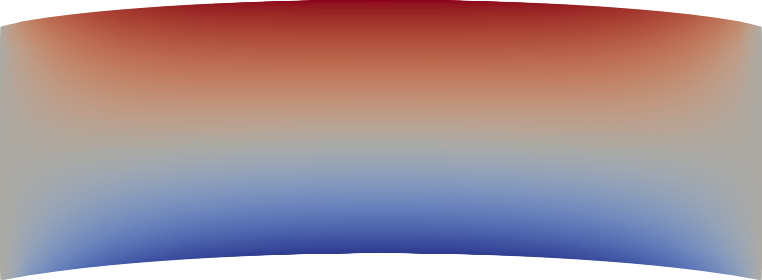
\includegraphics[width=6cm]{../03-thermo-elasto-static/01-sunshine/theta.png}};
  \begin{scope}[xshift=3.5cm,yshift=1.3cm,scale=0.5]
   \begin{axis}[verticalbar,point meta min=-6.16,point meta max=6.16,title={$\theta - \theta_0$ in $\mathrm{K}$}] 
    \addplot [draw=none] coordinates {(0,0)}; \end{axis}
  \end{scope}   
  }
  \onslide<3>{
  \node at(1.5,0.55) {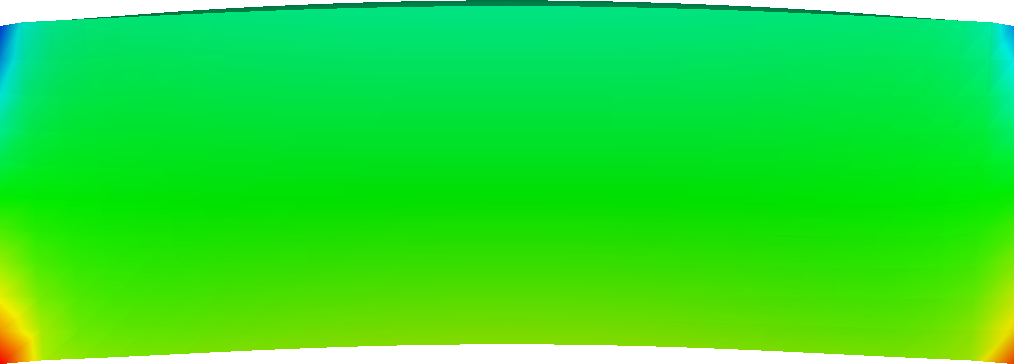
\includegraphics[width=6cm]{../03-thermo-elasto-static/01-sunshine/stress.png}};
  \begin{scope}[xshift=3.5cm,yshift=1.3cm,scale=0.5]
   \begin{axis}[verticalbar,point meta min=-50.2,point meta max=50.2,title={$\sigma_{11}$ in $\mathrm{MPa}$}] 
    \addplot [draw=none] coordinates {(0,0)}; \end{axis}
  \end{scope}   
  }

  \onslide<1-3>{
  \fill[pattern=north west lines, pattern color=black] (0, -0.25) rectangle +(-0.25, 1.5);
  \draw[thick] (0, -0.25) -- +(0, 1.5);
  \fill[pattern=north west lines, pattern color=black] (3, -0.25) rectangle +(0.25, 1.5);
  \draw[thick] (3, -0.25) -- +(0, 1.5);

  \fill[gray] (0.0, 0.0) rectangle +(-0.05, 1.0);
  \fill[gray] (3.0, 0.0) rectangle +(0.05, 1.0);

  }
  \onslide<1>{
  \draw (-0.25, 0.5) node[above, rotate=90] {$\theta^p=\theta_0$};
  \draw (3.25, 0.5) node[below, rotate=90] {$\theta^p=\theta_0$};
 }

  
  \begin{scope}
   \onslide<1>{\node at (0, -1.5) [right]{\parbox{3cm}{$E = 200 \, \mathrm{GPa}$ \\ $\nu = 0.3$ \\ $\ell = 0.1\,\mathrm{m}$}};}
   \onslide<1>{\node at (1.5, -1.5) [right]{\parbox{3cm}{$\kappa = 80 \, \frac{\mathrm{W}}{\mathrm{m}\cdot\mathrm{K}}$ \\ 
							 $\alpha = 15\cdot 10^{-6} \, \frac{1}{\mathrm{K}}$}};}
   \onslide<1>{\node at (3.2, -1.5) [right]{\parbox{4cm}{$q^p_\text{top} = 10 \, \frac{\mathrm{kW}}{\mathrm{m}^2}$ \\ 
							 $q^p_\text{bottom} = -10 \, \frac{\mathrm{kW}}{\mathrm{m}^2}$}};}
   \onslide<2-3>{\node at (0, -0.5) [right,font=\footnotesize]{$\v u$ scaled with a factor of $2000$};}
  \end{scope}
  
  \end{tikzpicture}
  \end{center}

 \end{overlayarea}
\end{frame}





\begin{frame}
 \frametitle{Demo 3-2 $\vert$ \bfseries Thermo-elasto-statics}
 \framesubtitle{\bfseries bimetallic thermometer}
 \begin{overlayarea}{0.9\textwidth}{0.9\textheight}
%  \vspace*{1ex}
 \begin{center}
 \begin{tikzpicture}[scale=2]
  \onslide<1>{
    \fill[gray!50] (0.0, 0.0) rectangle +(-0.05, 0.4);
  \fill[gray!50] (4.0, 0.0) rectangle +(0.05, 0.4);
  \fill[gray!50] (-0.05, 0.0) rectangle +(4.1, -0.05);
  \fill[gray!50] (-0.05, 0.4) rectangle +(4.1, 0.05);
  
  \fill[gray!10, draw=black] (0, 0.4) rectangle (4, 0) node[above left, yshift=-2pt, black]{$\mathcal{B}$};
  }

  \onslide<1>{
  \draw[thin,gray] (0, 0) -- +(0, -0.5);
  \draw[thin,gray] (4, 0) -- +(0, -0.5);
  \draw[<->,thin,gray] (0, -0.4) -- node[fill=white]{$3 \, \mathrm{cm}$} +(4, 0);
  \draw[thin,gray] (4, 0) -- +(0.5, 0);
  \draw[thin,gray] (4, 0.4) -- +(0.5, -0);
  \draw[<->,gray] (4.4, 0) -- node[fill=white]{$2 \, \mathrm{mm}$} +(0, 0.4);

   \draw[thick,-latex] (0,0) -- +(0.5, 0) node[below]{$\v e_1$};
   \draw[thick,-latex] (0,0) -- +(0, 0.5) node[right]{$\v e_2$};
  }
  
%   \onslide<1>{
%   \foreach \x in {0.0, 0.25,0.5,...,2.75, 3.0}{
%    \draw[decorate,decoration={snake, amplitude=1pt, segment length=5pt, post length=3pt},-latex] (0.05+2.9/3.0*\x, 1.5) -- +(0, -0.5);
%    \draw[decorate,decoration={snake, amplitude=1pt, segment length=5pt, post length=3pt},-latex] (0.05+2.9/3.0*\x, 0.0) -- +(0, -0.5);  
%   }
% %   \draw (0.05, 1.5) -- node[above]{$10 \,\mathrm{MPa}$} +(2.9, 0);
%   \node at (2.9, 1.5) [right,xshift=0.1cm]{$q^p_\text{top}$};
%   \node at (2.9, -0.5) [right,xshift=0.1cm]{$q^p_\text{bottom}$};
%   }

  \onslide<2>{
  \node at(2,-0.15) {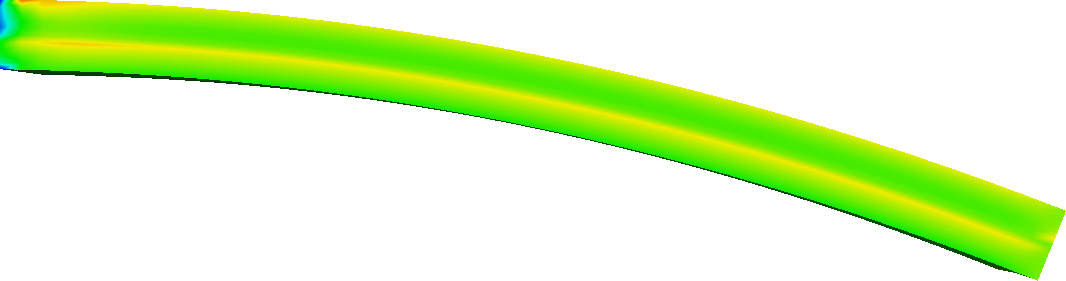
\includegraphics[width=8cm]{../03-thermo-elasto-static/02-bimetal/stress.png}};
  \begin{scope}[xshift=4cm,yshift=0.8cm,scale=0.5]
   \begin{axis}[verticalbar,point meta min=-110,point meta max=67,title={$\sigma_{11}$ in $\mathrm{MPa}$}] 
    \addplot [draw=none] coordinates {(0,0)}; \end{axis}
  \end{scope}   
  }

  \onslide<1-2>{
  \fill[pattern=north west lines, pattern color=black] (0, -0.25) rectangle +(-0.25, 0.9);
  \draw[thick] (0, -0.25) -- +(0, 0.9);
%   \fill[pattern=north west lines, pattern color=black] (3, -0.25) rectangle +(0.25, 1.5);
%   \draw[thick] (3, -0.25) -- +(0, 1.5);
  }
  \onslide<1>{
   \draw[dashed] (0, 0.2) -- +(4, 0);
   \node at (2, 0.3) {$\alpha_1$};
   \node at (2, 0.1) {$\alpha_2$};
   
   \node at (1.2, 0.4) [above]{$\theta^p = \theta_0 + 25 \, \mathrm{K}$};
   \node at (2.8, 0.0) [below]{$\theta^p = \theta_0 + 25 \, \mathrm{K}$};

 }

  
  \begin{scope}
   \onslide<1>{\node at (0, -1.5) [right]{\parbox{3cm}{$E = 200 \, \mathrm{GPa}$ \\ $\nu = 0.3$ \\ $\kappa = 80 \, \frac{\mathrm{W}}{\mathrm{m}\cdot\mathrm{K}}$}};}
   \onslide<1>{\node at (1.5, -1.5) [right]{\parbox{3cm}{$\alpha_1 = 15\cdot 10^{-6} \, \frac{1}{\mathrm{K}}$\\
							 $\alpha_2 = 1\cdot 10^{-6} \, \frac{1}{\mathrm{K}}$}};} %\\
							 %$\theta = \theta_0 + 25 \, \mathrm{K}$}};}
%    \onslide<1>{\node at (3.2, -1.5) [right]{\parbox{4cm}{$q^p_\text{top} = 10 \, \frac{\mathrm{kW}}{\mathrm{m}^2}$ \\ 
% 							 $q^p_\text{bottom} = -10 \, \frac{\mathrm{kW}}{\mathrm{m}^2}$}};}
   \onslide<2>{\node at (0, -0.5) [right,font=\footnotesize]{$\v u$ scaled with a factor of $50$};}
  \end{scope}
  
  \onslide<1>{
   \node at(4.5,-1.3) {
\includegraphics[width=3cm]{thermometer.jpg}};
   \node at(4.5,-2.1) {\parbox{3cm}{\tiny https://commons.wikimedia.org \\/w/index.php?curid=235662\\ CC BY-SA 3.0}};
  }
  
  \end{tikzpicture}
  \end{center}

 \end{overlayarea}
\end{frame}
